\scanpage{73}
% archive foliation: 75
(soit $U=f(\mathbb D^\circ)$)

\figure{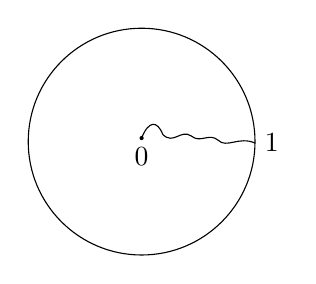
\begin{tikzpicture}[scale=.9]
\draw (0,0) circle (1.6);
\draw (0,.05) .. controls (.1,.3) and (.22,.3) .. (.3,.1)
 .. controls (.45,-.05) and (.55,.18) .. (.7,.08)
 .. controls (.83,-.03) and (.95,.13) .. (1.08,.02)
 .. controls (1.2,-.1) and (1.37,.08) .. (1.6,-.02);
\fill (0,.05) circle (.03);\node[below] at (0,.05) {$0$};
\node[right] at (1.6,-.02) {$1$};
\end{tikzpicture}}

2) $f(\unsure{\omega|0})=0$, $f(\zeta)=f(\overline\zeta)=1$

\deleted{\unsure{3)} $f|\beta$ est un}
$f|(\alpha\setminus\{\zeta,\overline\zeta\})$ \deleted{est}\inserted{induit} un
homéom avec $\delta\mathbb D\setminus\{1\}$

3) \deleted{$\unsure{f(\beta)=I}$} $f|\beta$ et $f|\overline\beta$ sont bijections et
ont $=$ image $\overline I$, \deleted{\unsure{qui est} et $\overline I\setminus\{1\}$}\inserted{contenant $\{1\}$} d'après
2), et $\overline I\setminus\{1\}$ est contenu dans $\mathbb D^\circ$.

4) Soient $f_1:\beta\overset\sim\longrightarrow\overline I$, $f_2:\overline\beta\overset\sim\longrightarrow\overline I$ induites par $f$,
alors $\varphi=f_2^{-1}f_1$

\uline{NB} De nouveau, $f$ est unique. On peut
résumer ce théorème d'uniformisation
au bord dans le \deleted{Scholie}

\uline{Scholie} Il y a corr. $1$-$1$ entre les
données suivantes :

a) Les homéom rectifiables \deleted{\unsure{en}}
\[
\psi:[0,1]\overset\sim-\,[0,1]
\qquad\text{avec }\psi(0)=0\quad(\text{donc }\psi(1)=1)
\]

b) Les segments topologiques \uline{rectifiables}
$\overline I$ dans $\mathbb D$, tels que
\deleted{$\overline I\cap\delta\mathbb D$ soit réduit}
\inserted{$\overline I$ admette $0,1$ comme}
extrémités et \deleted{$\unsure{\overline I\setminus\{1\}\subset\mathbb D}$}
$\overline I\cap\delta\mathbb D=\{1\}$ (i.e.
\deleted{à une extrémité de $\overline I$}
$\overline I\setminus\{1\}\subset\mathbb D^\circ$)

c) Les \deleted{\unsure{a}} applications continues $f:\mathbb D\longrightarrow\mathbb D$
qui ont les propriétés 1) 2) 3) de B) ci-dessus
